\paragraph{QuizziPedia::Front-End::Controllers::StatisticsController}
\begin{figure} [ht]
	\centering
	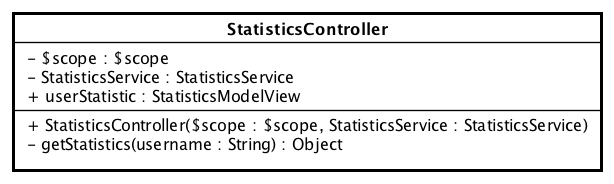
\includegraphics[scale=0.45]{UML/Classi/Front-End/QuizziPedia_Front-end_Controller_StatisticsController.png}
	\caption{QuizziPedia::Front-End::Controllers::StatisticsController}
\end{figure} \FloatBarrier
\begin{itemize}
	\item \textbf{Descrizione}: questa classe permette di le statistiche di un utente;
	\item \textbf{Utilizzo}: fornisce le funzionalità per ottenere le statistiche di un utente per poterle mostrare nella view;
	\item \textbf{Relazione con altre classi}:
	\begin{itemize}
		\item \textit{IN} \texttt{StatisticsModelView}: classe di tipo modelview la cui istanzazione è contenuta all'interno della variabile di ambiente \$scope di \textit{Angular.js\ped{G}}. All'interno di essa sono presenti le variabili e i metodi necessari per il \textit{Two-Way Data-Binding\ped{G}} tra la directive \texttt{StatisticsDirective} e il controller \texttt{StatisticsController}; 
		\item \textit{IN} \texttt{StatisticsService}: questa classe permette di ottenere le statistiche dell'utente;
	\end{itemize}
	\item \textbf{Attributi}:
	\begin{itemize}
		\item \texttt{-} \texttt{\$scope: \$scope} \\
		Campo dati contenente un riferimento all’oggetto \$scope creato da \textit{Angular\ped{G}}, viene utilizzato come mezzo di comunicazione tra il controller e la view. Contiene gli oggetti che definiscono il model dell’applicazione;
		\item \texttt{-} \texttt{StatisticsService: StatisticsService} \\
		Campo dati contenente un riferimento al servizio che si occupa della gestione delle informazioni legate alle statistiche da visualizzare;
	\end{itemize}	
	\begin{itemize}
		\item \textbf{Metodi}:
		\item \texttt{+} \texttt{StatisticsController(\$scope: \$scope, StatisticsService: StatisticsService)} \\ 
		Metodo costruttore della classe. \\
		\begin{itemize}
			\item \texttt{\$scope: \$scope} \\
			Parametro contenente un riferimento all’oggetto \$scope creato da \textit{Angular\ped{G}}. Viene utilizzato come mezzo di comunicazione tra il controller e la view. Contiene gli oggetti che definiscono il viewmodel e il model dell’applicazione;
			\item \texttt{StatisticsService: StatisticsService} \\
			Parametro contenente un riferimento al servizio che si occupa della gestione delle informazioni legate alle statistiche da visualizzare;
		\end{itemize}
		\item \texttt{+} \texttt{getStatistics(username: String)} \\ 
		Metodo che permette di ottenere le statistiche si un utente grazie all'utilizzo di \texttt{StatisticsService}; \\
		\textbf{Parametri}: 
		Metodo costruttore della classe. \\
		\begin{itemize}
			\item \texttt{username: String} \\
			Parametro contenente la stringa username utilizzata per poter recuperare le giuste statistiche attraverso lo \texttt{StatisticsService}; 
		\end{itemize}
	\end{itemize}
\end{itemize}

